\hypertarget{acpy3_8h}{
\subsection{acpy3.h File Reference}
\label{acpy3_8h}\index{acpy3.h@{acpy3.h}}
}


\subsubsection{Detailed Description}
ACPY3 Definitions (C64P) - 3rd Generation ACPY. Provides a comprehensive list of DMA operations an algorithm can perform on logical DMA channels it acquires through the IDMA3 protocol. 



Definition in file \hyperlink{acpy3_8h-source}{acpy3.h}.

{\tt \#include $<$ti/xdais/idma3.h$>$}\par


Include dependency graph for acpy3.h:\begin{figure}[H]
\begin{center}
\leavevmode
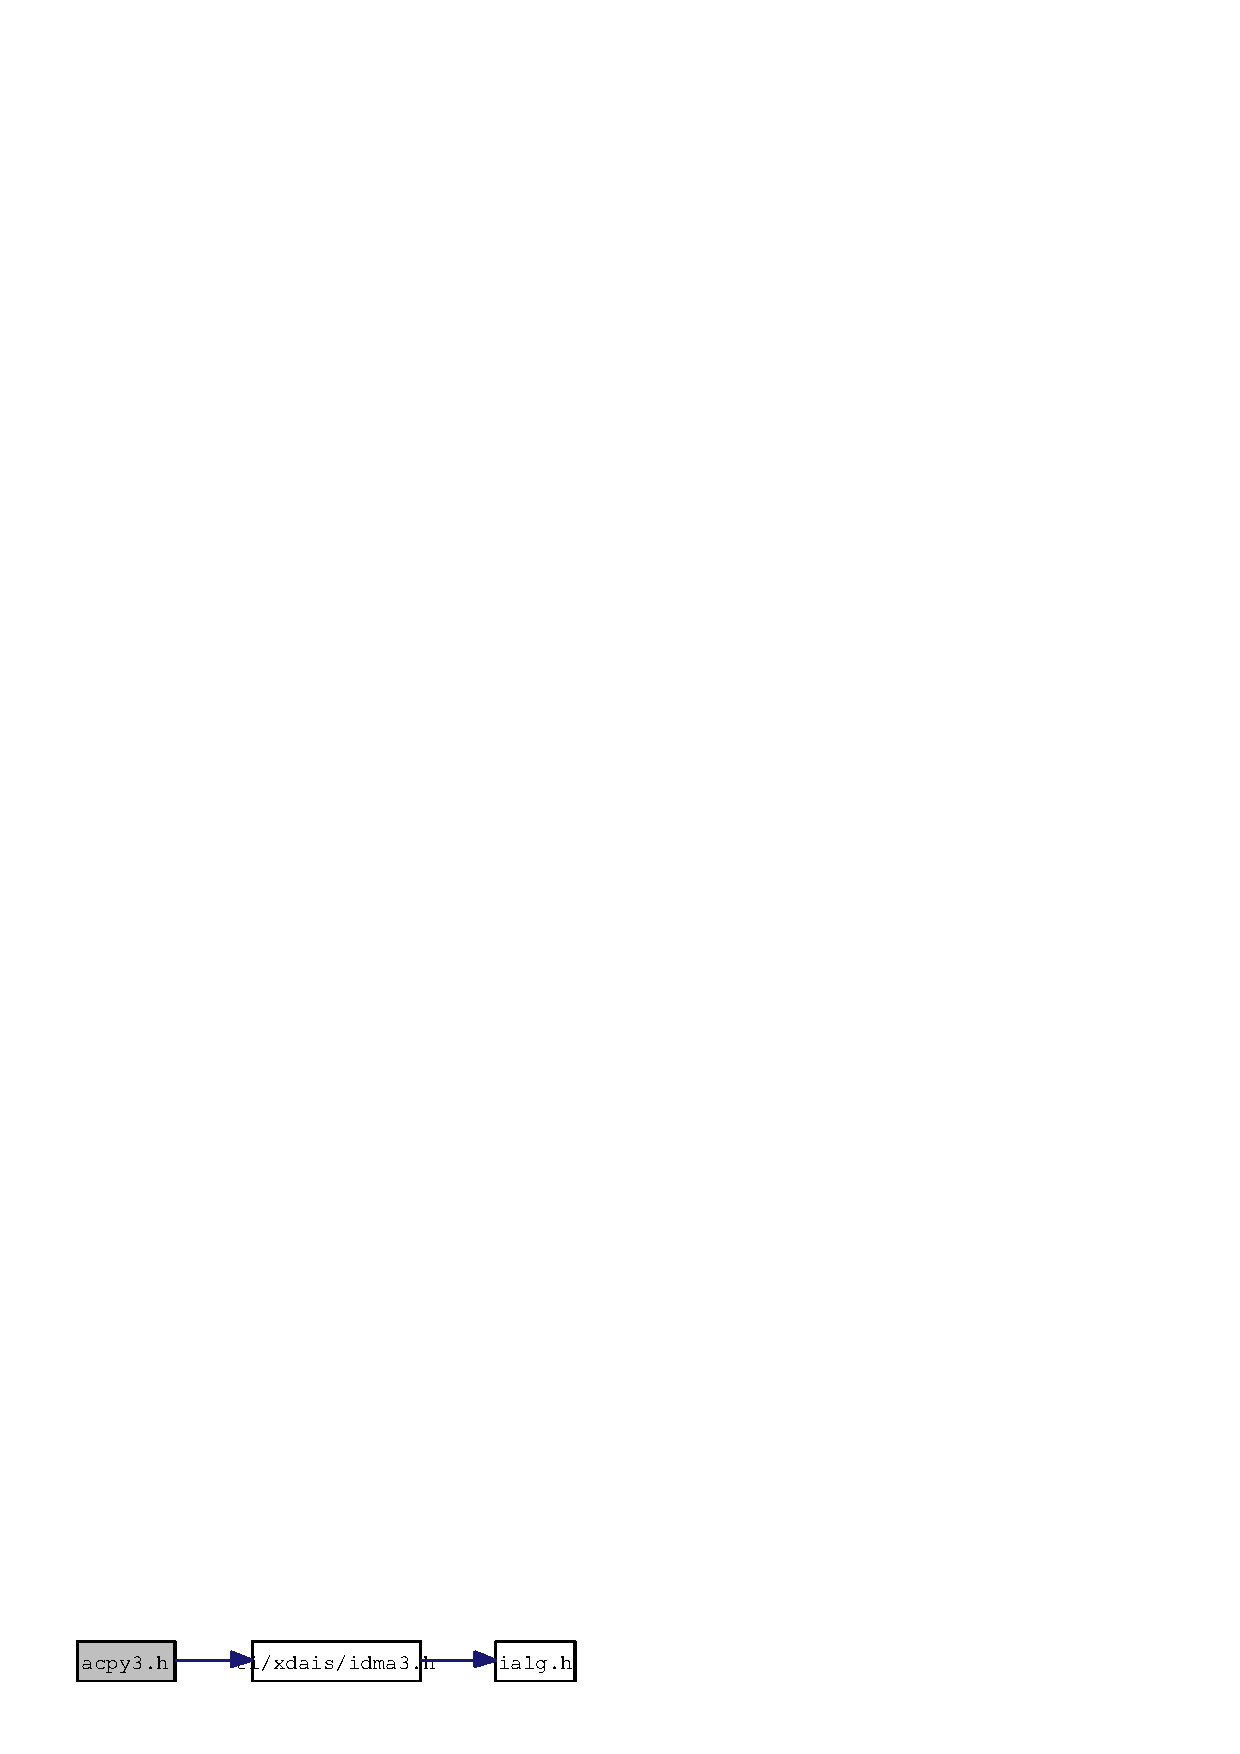
\includegraphics[width=138pt]{acpy3_8h__incl}
\end{center}
\end{figure}
\subsubsection*{Data Structures}
\begin{CompactItemize}
\item 
struct \hyperlink{struct_a_c_p_y3___params}{ACPY3\_\-Params}
\begin{CompactList}\small\item\em DMA transfer specific parameters. Defines the configuration of a logical channel. \item\end{CompactList}\end{CompactItemize}
\subsubsection*{Enumerations}
\begin{CompactItemize}
\item 
enum \hyperlink{group___d_s_p_a_c_p_y3_gf9624d3d925ec0d15bd845967664e608}{ACPY3\_\-Param\-Field16b} \{ \par
\hyperlink{group___d_s_p_a_c_p_y3_ggf9624d3d925ec0d15bd845967664e608f590c76a022dbe56043c8a0a577a88c8}{ACPY3\_\-PARAMFIELD\_\-ELEMENTSIZE} =  8, 
\par
\hyperlink{group___d_s_p_a_c_p_y3_ggf9624d3d925ec0d15bd845967664e608b95b07e80a06c8d2b0ccd191de1fb8aa}{ACPY3\_\-PARAMFIELD\_\-NUMELEMENTS} =  10, 
\par
\hyperlink{group___d_s_p_a_c_p_y3_ggf9624d3d925ec0d15bd845967664e608a3a4872acfc89e4da1820e0839b0fb87}{ACPY3\_\-PARAMFIELD\_\-ELEMENTINDEX\_\-SRC} =  16, 
\par
\hyperlink{group___d_s_p_a_c_p_y3_ggf9624d3d925ec0d15bd845967664e608a1c08ec69ae102d758b8678c492038e3}{ACPY3\_\-PARAMFIELD\_\-ELEMENTINDEX\_\-DST} =  18, 
\par
\hyperlink{group___d_s_p_a_c_p_y3_ggf9624d3d925ec0d15bd845967664e608cd1fe7c99a4596d8724a9cf359bf8f57}{ACPY3\_\-PARAMFIELD\_\-FRAMEINDEX\_\-SRC} =  24, 
\par
\hyperlink{group___d_s_p_a_c_p_y3_ggf9624d3d925ec0d15bd845967664e608ad2460b82b3834e625dcdb3e1e2c140c}{ACPY3\_\-PARAMFIELD\_\-FRAMEINDEX\_\-DST} =  26, 
\par
\hyperlink{group___d_s_p_a_c_p_y3_ggf9624d3d925ec0d15bd845967664e6085593f2242b7d6741c9dcb4233909942d}{ACPY3\_\-PARAMFIELD\_\-NUMFRAMES} =  28
 \}
\begin{CompactList}\small\item\em ACPY3 16-bit param field structure. These values are passed to \hyperlink{group___d_s_p_a_c_p_y3_g2c54ca4dc3d0cf3f861259bc7cf0f8de}{ACPY3\_\-fast\-Configure16b()} to indicate the field of the \hyperlink{struct_a_c_p_y3___params}{ACPY3\_\-Params} structure to be changed. \item\end{CompactList}\item 
enum \hyperlink{group___d_s_p_a_c_p_y3_g96f43d4bc010da2d1bb9dc08ea828de0}{ACPY3\_\-Param\-Field32b} \{ \par
\hyperlink{group___d_s_p_a_c_p_y3_gg96f43d4bc010da2d1bb9dc08ea828de0807013269912df7c5dbc2361483d2e1e}{ACPY3\_\-PARAMFIELD\_\-SRCADDR} =  4, 
\par
\hyperlink{group___d_s_p_a_c_p_y3_gg96f43d4bc010da2d1bb9dc08ea828de0927624fccb072b2ff847a10c4729fedf}{ACPY3\_\-PARAMFIELD\_\-DSTADDR} =  12, 
\par
\hyperlink{group___d_s_p_a_c_p_y3_gg96f43d4bc010da2d1bb9dc08ea828de0ce2eb39c83c77fa1ee38d5c87e045e83}{ACPY3\_\-PARAMFIELD\_\-ELEMENTINDEXES} =  16, 
\par
\hyperlink{group___d_s_p_a_c_p_y3_gg96f43d4bc010da2d1bb9dc08ea828de088347f099298128f5989f76636e64dc5}{ACPY3\_\-PARAMFIELD\_\-FRAMEINDEXES} =  24
 \}
\begin{CompactList}\small\item\em ACPY3 32-bit param field structure. These values are passed to \hyperlink{group___d_s_p_a_c_p_y3_g2ad7ed5dc554a991c4c11f644f5a8272}{ACPY3\_\-fast\-Configure32b()} to indicate the field of the \hyperlink{struct_a_c_p_y3___params}{ACPY3\_\-Params} structure to be changed. \item\end{CompactList}\item 
enum \hyperlink{group___d_s_p_a_c_p_y3_gbe2d02fcbde983c823b138f20667cbfc}{ACPY3\_\-Transfer\-Type} \{ \par
\hyperlink{group___d_s_p_a_c_p_y3_ggbe2d02fcbde983c823b138f20667cbfcf9cef75ab1829399370006a48d16182e}{ACPY3\_\-1D1D}, 
\par
\hyperlink{group___d_s_p_a_c_p_y3_ggbe2d02fcbde983c823b138f20667cbfc7e3376fb0def5e38484dfb121e7b2fb7}{ACPY3\_\-1D2D}, 
\par
\hyperlink{group___d_s_p_a_c_p_y3_ggbe2d02fcbde983c823b138f20667cbfc3ad50651b016c2c96f8fb6f724213623}{ACPY3\_\-2D1D}, 
\par
\hyperlink{group___d_s_p_a_c_p_y3_ggbe2d02fcbde983c823b138f20667cbfcd8ac84d79831cfe53a4088a321989a85}{ACPY3\_\-2D2D}
 \}
\begin{CompactList}\small\item\em ACPY3 DMA Transfer Types:. \item\end{CompactList}\end{CompactItemize}
\subsubsection*{Functions}
\begin{CompactItemize}
\item 
Void \hyperlink{group___d_s_p_a_c_p_y3_g427e8e4fd5c445b2f9bb5d971c06c099}{ACPY3\_\-configure} (\hyperlink{struct_i_d_m_a3___obj}{IDMA3\_\-Handle} handle, \hyperlink{struct_a_c_p_y3___params}{ACPY3\_\-Params} $\ast$params, Md\-Int transfer\-No)
\begin{CompactList}\small\item\em Functions called by the framework for allocating and initializing the channel state. Configure all DMA transfer settings for the logical channel. \item\end{CompactList}\item 
Void \hyperlink{group___d_s_p_a_c_p_y3_g2c54ca4dc3d0cf3f861259bc7cf0f8de}{ACPY3\_\-fast\-Configure16b} (\hyperlink{struct_i_d_m_a3___obj}{IDMA3\_\-Handle} handle, \hyperlink{group___d_s_p_a_c_p_y3_gf9624d3d925ec0d15bd845967664e608}{ACPY3\_\-Param\-Field16b} field\-Id, Md\-Uns value, Md\-Int transfer\-No)
\begin{CompactList}\small\item\em Modify the 16-bit DMA transfer parameter, indicated by the parameter field id, field\-Id, of the current channel settings. \item\end{CompactList}\item 
Void \hyperlink{group___d_s_p_a_c_p_y3_g2ad7ed5dc554a991c4c11f644f5a8272}{ACPY3\_\-fast\-Configure32b} (\hyperlink{struct_i_d_m_a3___obj}{IDMA3\_\-Handle} handle, \hyperlink{group___d_s_p_a_c_p_y3_g96f43d4bc010da2d1bb9dc08ea828de0}{ACPY3\_\-Param\-Field32b} field\-Id, Uns value, Md\-Int transfer\-No)
\begin{CompactList}\small\item\em Modify the 32-bit DMA transfer parameter, indicated by the parameter field id, field\-Id, of the current channel settings. \item\end{CompactList}\item 
Void \hyperlink{group___d_s_p_a_c_p_y3_gfc7ddb15d68ef3741abfb8843763fce5}{ACPY3\_\-set\-Final} (\hyperlink{struct_i_d_m_a3___obj}{IDMA3\_\-Handle} handle, Md\-Int transfer\-No)
\begin{CompactList}\small\item\em Indicate that a given transfer will be the last in a sequence of linked transfers. \item\end{CompactList}\item 
Void \hyperlink{group___d_s_p_a_c_p_y3_g44f2ce173d41bc7bbfb6e7fb500ec58f}{ACPY3\_\-fast\-Set\-Final} (\hyperlink{struct_i_d_m_a3___obj}{IDMA3\_\-Handle} handle, Md\-Int transfer\-No)
\begin{CompactList}\small\item\em Indicate that a given transfer will be the last in a sequence of linked transfers. \item\end{CompactList}\item 
Void \hyperlink{group___d_s_p_a_c_p_y3_gb4102200f00a9df3961a8374c0042bed}{ACPY3\_\-start} (\hyperlink{struct_i_d_m_a3___obj}{IDMA3\_\-Handle} handle)
\begin{CompactList}\small\item\em Submit a single or linked transfer using the most recently configured transfer parameter settings. \item\end{CompactList}\item 
Void \hyperlink{group___d_s_p_a_c_p_y3_g499bc0643a52f5cfd0828c1ce21cd69b}{ACPY3\_\-wait} (\hyperlink{struct_i_d_m_a3___obj}{IDMA3\_\-Handle} handle)
\begin{CompactList}\small\item\em Wait for all data transfers on a logical channel to complete. \item\end{CompactList}\item 
Void \hyperlink{group___d_s_p_a_c_p_y3_g6acf0b26cee48d5cbc81e2c9049128ea}{ACPY3\_\-wait\-Linked} (\hyperlink{struct_i_d_m_a3___obj}{IDMA3\_\-Handle} handle, Md\-Uns wait\-Id)
\begin{CompactList}\small\item\em Wait for an individual transfer in a Linked transfer to finish. \item\end{CompactList}\item 
Bool \hyperlink{group___d_s_p_a_c_p_y3_ge22deca1f6878a359a619cff8654d9de}{ACPY3\_\-complete} (\hyperlink{struct_i_d_m_a3___obj}{IDMA3\_\-Handle} handle)
\begin{CompactList}\small\item\em Check to see if all dma transfers on logical channel are finished. \item\end{CompactList}\item 
Bool \hyperlink{group___d_s_p_a_c_p_y3_g88a22e18670a97816b27dcd90abf2ae9}{ACPY3\_\-complete\-Linked} (\hyperlink{struct_i_d_m_a3___obj}{IDMA3\_\-Handle} handle, Md\-Uns wait\-Id)
\begin{CompactList}\small\item\em Non-blocking query to check completion of an individual transfer in a Linked transfer. \item\end{CompactList}\item 
Void \hyperlink{group___d_s_p_a_c_p_y3_gf9dc07965774895d79323a47b36cc442}{ACPY3\_\-activate} (\hyperlink{struct_i_d_m_a3___obj}{IDMA3\_\-Handle} handle)
\begin{CompactList}\small\item\em Activate the given channel. \item\end{CompactList}\item 
Void \hyperlink{group___d_s_p_a_c_p_y3_g2736d2e136e868577a71710571027de5}{ACPY3\_\-deactivate} (\hyperlink{struct_i_d_m_a3___obj}{IDMA3\_\-Handle} handle)
\begin{CompactList}\small\item\em Deactivates the given channel. \item\end{CompactList}\item 
Void \hyperlink{group___d_s_p_a_c_p_y3_gc79227aad8cb9f68ab67da77de81fd17}{ACPY3\_\-init} (Void)
\begin{CompactList}\small\item\em Initialize the ACPY3 module. Called by framework. \item\end{CompactList}\item 
Void \hyperlink{group___d_s_p_a_c_p_y3_ge7072f7010b53bdeab5ac76737b380af}{ACPY3\_\-exit} (Void)
\begin{CompactList}\small\item\em Finalization of the ACPY3 module. \item\end{CompactList}\end{CompactItemize}
\subsubsection*{Variables}
\begin{CompactItemize}
\item 
\hyperlink{struct_i_d_m_a3___protocol_obj}{IDMA3\_\-Protocol\-Obj} \hyperlink{group___d_s_p_a_c_p_y3_g7171d01619b7fc26dbb11eb9aaf1a3b2}{ACPY3\_\-PROTOCOL}
\end{CompactItemize}
